\documentclass[tikz]{standalone}%

\usepackage[utf8]{inputenx}%  http://ctan.org/pkg/inputenx
% Euler for math | Palatino for rm | Helvetica for ss | Courier for tt
\renewcommand{\rmdefault}{ppl}% rm
\linespread{1.05}% Palatino needs more leading
\usepackage[scaled]{helvet}% ss //  http://ctan.org/pkg/helvet
\usepackage{courier}% tt // http://ctan.org/pkg/courier
\usepackage{eulervm}  %  http://ctan.org/pkg/eulervm
% a better implementation of the euler package (not in gwTeX)
\normalfont%
\usepackage[T1]{fontenc}%  http://ctan.org/pkg/fontenc
\usepackage{textcomp}%  http://ctan.org/pkg/textcomp

\usetikzlibrary{patterns}
\usetikzlibrary{calc}

\begin{document}
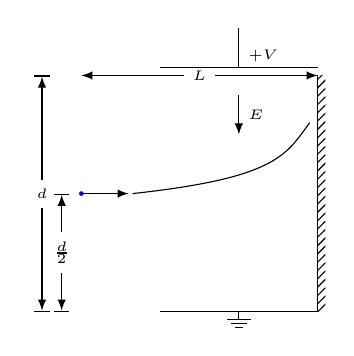
\begin{tikzpicture}
  \fill[pattern = north east lines] (2, 0) coordinate (P1) rectangle (2.1, 3)
  coordinate (P2) at (2, 3);

  \draw (0, 0) coordinate (O) -- (P1) -- (P2);
  \draw[latex-latex] (P2) -- +(-3, 0) node[pos = .5, fill = white,
  font = \tiny] {$L$};
  \draw[>=latex, |<->|] (-1.5, 0) -- (-1.5, 3) node[font = \tiny, pos = .5,
  fill = white] {$d$};
  \draw[>=latex, |<->|] (-1.25, 0) -- (-1.25, 1.5) node[font = \tiny,
  pos = .5, fill = white] {$\frac{d}{2}$};

  \draw[-latex] (-1, 1.5) -- +(.6, 0) coordinate (P3);
  \draw ($(P3) + (.05, 0)$) .. controls (1.5, 1.7) and (1.6, 2) .. (1.9, 2.4);
  \draw (1, 0) -- +(0, -0.1);
  \draw (0.85, -0.1) -- +(0.3, 0);
  \draw (0.9, -0.15) -- +(0.2, 0);
  \draw (0.95, -0.2) -- +(0.1, 0);
  \draw[-latex] (1, 2.75) -- +(0, -0.5) node[right, pos = .5, font = \tiny]
  {$E$};
  \draw (2, 3.1) -- (0, 3.1);
  \draw (1, 3.1) -- +(0, .5) node[pos = .3, right, font = \tiny] {$+V$};
  
  \fill[blue] (-1, 1.5) circle[radius = .03cm];
\end{tikzpicture}
\end{document}
%%% Local Variables:
%%% mode: latex
%%% TeX-master: t
%%% End:
